
\lecture{Indução Matemática}{induction}

\begin{frame}{\insertlecture}
  
  Seja $P(n)$ uma afirmação sobre um inteiro $n$. Supondo que queremos
  provar que $P(n)$ é verdadeira para todos os inteiros positivos. Um 
  modo fundamental de fazer isto é:

  \begin{enumerate}
  \item Fornecer um prova de que $P(1)$ é verdadeira;
  \item Fornecer uma prova de que se $P(1), P(2), \dots, P(n)$ são 
    verdadeiras, então $P(n+1)$ também é verdadeira; e esta prova deve
    ser válida para todos os inteiros positivos.
  \end{enumerate}
\end{frame}

\begin{frame}{Exemplo de indução matemática}
Considere as seguintes séries de equações.\\

\[  
  \begin{array}{c}
    1=1^2 \\
    1+3=2^2\\
    1+3+5 = 3^2\\
    1+3+5+7 = 4^2\\
    1+3+5+7+9 = 5^2
  \end{array}
\]

\pause

Podemos formular a seguinte propriedade geral:\\

\begin{equation}
1+3+\dots+(2n-1) = n^2
\label{eq:induction:example}
\end{equation}

\end{frame}

\begin{frame}{Prova do exemplo de indução matemática}
  \begin{enumerate}
  \item<1-> P(1) é verdadeira, pois, $1=1^2$;
  \item<2> Se todas $P(1),\dots,P(n)$ são verdadeiras, então, 
    em particular, $P(n)$ é verdadeira, de modo que a 
    Eq.~(\ref{eq:induction:example}) sejá válida. Adicionando
    $2n+1$ em ambos os lados obtemos
    
    \[ 1+3+\dots+(2n-1)+(2n+1)=n^2+ 2n+1=(n+1)^2\]

  \bigskip
  que prova que $P(n+1)$ também é válida.
\end{enumerate}
\end{frame}

\begin{frame}{Algoritmo da prova por indução matemática}
  \def\dx{1.75cm}
  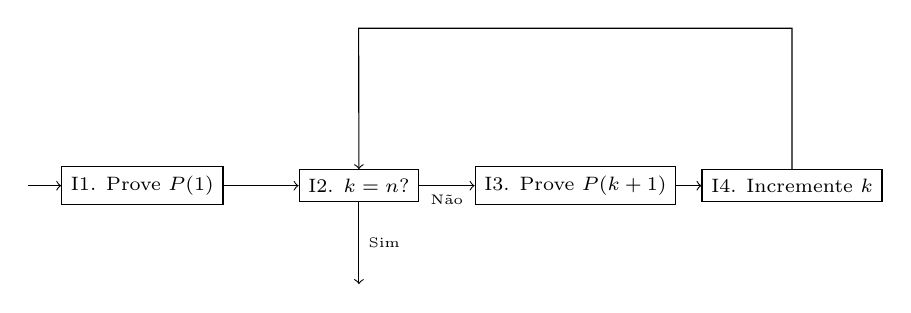
\begin{tikzpicture}[pstep/.style={font=\scriptsize,draw}]
    \node[pstep] (I1) [xshift=\dx] {I1. Prove $P(1)$};
    \node[pstep] (I2) [right of=I1,xshift=\dx] {I2. $k=n$?};
    \node[pstep] (I3) [right of=I2,xshift=\dx] {I3. Prove $P(k+1)$};
    \node[pstep] (I4) [right of=I3,xshift=\dx] {I4. Incremente $k$};
    
    \path[<-,draw] (I1) -- +(-1.45,0);
    \path[->,draw] (I1) -- (I2);
    \path[->,draw] (I2) -- node[anchor=north] {\tiny Não} (I3);
    \path[->,draw] (I3) -- (I4);
    \path[->,draw] (I4) -- +(0,2) -- +(-3.145*\dx,2) -- (I2); 
    \path[->,draw] (I2) -- node[font=\tiny,anchor=west] {Sim} +(0,-1.25);

  \end{tikzpicture}
\end{frame}
